\documentclass[journal]{IEEEtran}
\usepackage{cite}
% *** GRAPHICS RELATED PACKAGES ***
%
\ifCLASSINFOpdf
  \usepackage[pdftex]{graphicx}
\fi
%
\usepackage[cmex10]{amsmath}


% *** ALIGNMENT PACKAGES ***
%
\usepackage{array}
\usepackage{fixltx2e}

\usepackage{stfloats}
% LaTeX2e). It also provides a command:
\fnbelowfloat

\usepackage{amssymb}
\usepackage{amsmath}
\usepackage{pgf}
\usepackage{tikz}
\usetikzlibrary{arrows,positioning}
\usepackage{url}
\usepackage{color}
\usepackage{graphicx}
\usepackage{xspace}
\newcommand*{\eg}{e.g.\@\xspace}
\newcommand*{\ie}{i.e.\@\xspace}
\newcommand*{\vs}{vs.\@\xspace}

% correct bad hyphenation here
\hyphenation{op-tical net-works semi-conduc-tor}

\usepackage{color}
\newcommand{\vl}[1]{\textcolor{orange}{Vincent : #1}}
\newcommand{\gl}[1]{\textcolor{red}{Gr\'egoire : #1}}
\newcommand{\ja}[1]{\textcolor{magenta}{Joakim : #1}}
\newcommand{\ml}[1]{\textcolor{blue}{ Mathieu : #1}}



\begin{document}
%
% paper title
% can use linebreaks \\ within to get better formatting as desired
% Do not put math or special symbols in the title.
%\title{An evaluation framework for event detection using a morphological model of acoustic scenes}
\title{Object-based Auditory Scenes Similarity Retrieval and Classification With Scattering Transforms}

\author{Vincent Lostanlen, Gr\'egoire Lafay, Joakim And\'en, and Mathieu Lagrange}


% make the title area
\maketitle

% As a general rule, do not put math, special symbols or citations
% in the abstract or keywords.
\begin{abstract}
This paper introduces a generic hierarchical modeling of acoustic scenes using time/frequency scattering features for time spans below the second and object-based segmentation for larger time spans that effectiely model the scene with almost no requirement for optimization. Application of the proposed approach to the acoustic scene similarity and acoustic scene classification tasks demonstrates its potential.   

More precisely, the proposed approach achieves 
\end{abstract}

% Note that keywords are not normally used for peerreview paper.
\begin{IEEEkeywords}
Acoustic scene classification, acoustic scene segmentation.
\end{IEEEkeywords}

% For peer review papers, you can put extra information on the cover
% page as needed:
% \ifCLASSOPTIONpeerreview
% \begin{center} \bfseries EDICS Category: 3-BBND \end{center}
% \fi
%
% For peerreview papers, this IEEEtran command inserts a page break and
% creates the second title. It will be ignored for other modes.
\IEEEpeerreviewmaketitle

\section{Introduction}

\IEEEPARstart{O}{ver} the past decades, the amount of audio data recorded from our sonic environment has considerably grown. Recent research areas such as eco-acoustics \cite{ECOACOUSTICS2014, krause} start to consider massive deployment of acoustic sensors around the world in order to measure potential animal biodiversity modification over large temporal scales due to human activity or climate change \cite{NessSST13, stowell13a, stowell13b}. 

Also, some recent works demonstrate the interest of such approaches for the characterization of human acoustic pleasantness in urban areas \cite{lafayPartI, guyot2005urban, ricciardi2015sound} and the prediction of annoyance due to the traffic \cite{gloaguen}. We believe that those case study are of interest for the signal processing community as they have strong societal impacts and raises interesting research avenues. 

Unfortunately, those fields of research are still in infancy and consequently very few well built datasets are readily available for evaluation purposes for the signal processing community. A closely related field of investigation that is relatively more mature is the classification of acoustic scenes whose aim is to predict labels by processing audio data. Despite being narrower in terms of range of applications, it has the advantage of being rooted by numerous works in cognitive psychology on categorization \cite{dubois2006cognitive, maffiolo_caracterisation_1999, guastavino_ideal_2006} and been considered in the data processing field for a while, with availability of some well designed evaluation datasets. 

Despite the differences, the following question is valid both for the above cited future application and the acoustic scene classification (ASC) task. How can we efficiently and effectively process large amount of audio data using representations that are both compact, generic in their design and with a large application range ?  

The research described in this paper tackles that question by demonstrating the usefulness of two main contributions: 1) the use of the scattering transform allows us to extract discriminative features with almost no parameter optimization and 2) object-based modeling of the acoustic scene based on individual unsupervised clustering of each acoustic scene  allows us to effectively focus the description on areas of interest. After studying the state of the art in the field of acoustic scene modeling in Section \ref{sec:soa}, those contributions are extensively described, respectively in Section \ref{sec:scattering} and \ref{sec:object} and evaluated both in an unsupervised setting, \textit{i.e.} acoustic scene similarity (ASS) and in a supervised setting, \textit{i.e.}  acoustic scene classification (ASC), respectively in Section \ref{sec:similarity} and Section \ref{sec:classification}.

\section{Previous work} \label{sec:soa}

As stated in the introduction, the field of eco-acoustics is relatively young, but significant works are worth mentioning. One avenue of research issued from bio acoustic studies, consider the audio stream as a set of events produced animals, and is processed to retrieve the precise species that produced the sound and potentially the type of vocalization in order to predict some behavior of the animal under study \cite{dan}. Another, more recent, avenue of research, process the audio stream in an holistic manner in order to infer large time-scale properties of the bio-acoustic scene for example to estimate which part of the stream need to be analyzed in details, \textit{i.e.} by a human \cite{australians}.

The same dichotomy applies for the field of audio scene analysis, where the interest can be whether 1) to isolate and identify precise events, \textit{i.e.} acoustic event detection (AED) or 2) to predict global attributes assigned to large time spans of audio, \textit{i.e.} ASC. For the latter, most state-of-the-art systems roughly follow the bag of frame approach (BOF) initiated in \cite{aucouturier2007bag} where the audio is modelled as high level statistics comptued from a set of local features. Even though this approach as the advantage of high genericity and follows some evidence found by psycho perception research \cite{macdermott}, for the specific implementation with gaussian mixture models (GMMs) of Mel-frequency cepstral coefficients (MFCCs) it is demonstrated to be equivalent to  \cite{lagrange:hal-01082501}.

citer papier event based de l'intro de jj

 there is evidence that modelling the scene as a set of events allows us to predict high level semantic information such as pleasantness

Eventhough the precise list of events that occur in a given time is unachievable to get even for trained human, research shows that using only a few events, so called markers \cite{} is enough to reliably predict high level attributes. For example, the presence of a few bird calls in a smooth traffic hubhub is likely to be tagged by humans as a park scene in urban areas \gl{citations ?}.


\gl{DCASE challenge:} \cite{chum2013ieee}: CHR system, using HMM and frame based classification. \cite{elizalde2013vector} ELF system, I vector approach using probabilistic LDA as classifier. \cite{geiger2013large} GSR system, basically mel/MFCC using SVM as classifier. \cite{krijnders2013tone} KH system, tone fit features computed from cochleogram (but similar results are obtained with MFCCs) using SVM as classifier. \cite{li2013auditory} LTT system, Tree bagger classifier used on segments (MFCCs) before a majority vote. \cite{lee2013acoustic} NHL system, unsupervised feature learning approach on mel frequency spectrogram with selective Max-pooling. Supervised training is performed using SVM. \cite{nogueira2013sound} NR1 system, MFCC and spatial features (inter-aural differences) with SVM as classifier. \cite{olivetti2013wonder} OE system, normalized compression distance (I honestly did not understand a thing about it, but this the worst method of the challenge anyway) using  Random Forest  classifier.  \cite{patil2013multiresolution} PE system, 2D Gabor filters applied on 1sec segments with SVM as classifier.  \cite{rakotomamonjy2015histogram} RG system, histogram of gradient representation, computed from a constant Q transform with SVM as classifier.  \cite{roma2013recurrence} RNH system, RQA stacked with MFCC, SVM as classifier. \\

\gl{Other paper:} \cite{jiang2005svm, kalinli2009saliency, su2011environmental, barchiesi2015acoustic, ye2015acoustic, bisot2015hog, chakrabarty2015exploring, xue2015auditory, bisot2016acoustic}

\subsection{Describing a scene (Feature extraction)}

\subsection{Classifying a scene}

\subsection{Datasets}

defreville \cite{aucouturier2007bag}

\cite{lagrange:hal-01082501}

DCASE 2013 challenge reference papers. \cite{giannoulis2013database, 7100934} \\

For each scene type, three different recordists (DG, DS,
EB) visited a wide variety of locations in Greater London over
a period of months (Summer and Autumn 2012), and in each
scene recorded a few minutes of audio. We ensured that no
systematic variations in the recordings covaried with scene
type: all recordings were made in moderate weather condi-
tions, and varying times of day and week, and each recordist
recorded each scene type.

Rouen \cite{rakotomamonjy2015histogram}

\url{https://sites.google.com/site/alainrakotomamonjy/home/audio-scene}

dCase2016 \cite{Mesaros2016_EUSIPCO}

advantages of dcase2013:

controled intra class diversity

despite its size, it is still challenging as state-of-the-art systems achieves 76 \% \cite{roma2013} (winner of the 2013 challenge RQA+SVM). For the sake of comparison the HOG+SVM approach \cite{rakotomamonjy2015histogram} achieves 75 \% and 92 \% on the dcase2013 and the Rouen datasets respectively. On the latter, the state-of-the-art is currently 95 \% \cite{bisot2016acoustic}.

\section{Scattering representations \label{sec:scattering}}
Scattering transforms are translation-invariant representations of audio signals which cascade an auditory filterbank and a modulation filterbank, interspersed with complex modulus nonlinearities.
Depending upon the chosen architecture, the modulation filterbank may either be performed solely over the time variable or on both time and frequency variables.
In this section, we present both the temporal scattering transform and the time-frequency scattering transform.

\subsection{Invariance and stability in acoustic scene classification}
The notion of invariance to translation plays an essential role in auditory scene classification.
Indeed, the starting time of the recordings are chosen arbitrarily, and thus do not convey any information about the class.
To cancel this superfluous source of variability, signals must be mapped to a translation-invariant feature space before training the classifier.
From any set of descriptors -- \eg the time-frequency representation $\boldsymbol{x_1}(t,\gamma_1)$ of  a signal $\boldsymbol{x}(t)$ --
a translation-invariant representation up to time shifts of duration $T$ can be simply obtained
by convolving $\boldsymbol{x_1}$ with a low-pass filter $\boldsymbol{\phi}(t)$ of cutoff frequency
set to $1/T$:
\begin{equation}
\mathbf{S_1}\boldsymbol{x}(t, \gamma_1) = (\boldsymbol{x_1} \ast \boldsymbol{\phi}) (t).
\end{equation}
As a downside, the transient information in $\boldsymbol{x_1}$ at finer scales than $T$ are lost by this low-pass filtering, hence a lack of discriminability in feature space.
To address this issue, the temporal scattering transform recovers this information by convolving $\boldsymbol{x_1}$ with wavelets whose center frequencies are above $1/T$, and subsequently applying complex modulus.

By resorting to wavelet transform modulus, as opposed to Fourier transform modulus, the resulting features are provably stable to small time warps,
in the sense of Lipschitz regularity with respect to diffeomorphisms \cite{Mallat2012}.
Besides invariance to translation, this stability property is crucial in signal classification, as it entails a guarantee of robustness to small variations in pitch, reverberation, and rhythmic organization of events, which make up an important part of the intra-class variability among natural sounds.

The scattering transform is defined mathematically as an infinite cascade of nonlinear layers, each consisting of a wavelet transform modulus operator.
In practice, to achieve invariance to translation up to $T = 186\,\mathrm{ms}$, \ie of the order of the minimal duration between non-overlapping acoustic events, two layers of scattering transform of the audio signal $\boldsymbol{x}(t)$ suffice.

The next subsection describes the operations involved in temporal scattering.

\subsection{Temporal scattering}
Let $\boldsymbol{\psi}(t)$ a complex-valued band-pass filter of
center frequency $\xi_1$ and bandwidth $\xi_1/Q_1$.
A filter bank of wavelets is built by dilating $\boldsymbol{\psi}(t)$
according to a geometric sequence of scales $2^{\gamma_1/Q_1}$.
The variable $\gamma_1$, akin to a log-frequency, takes integer values between $0$ and $(J_1 \times Q_1 - 1)$.
In the sequel, we set $\xi_1$ to 20 kHz, \ie close to the Nyquist frequency of audio recordings ; the number of octaves $J_1$ to $10$, \ie the maximum range of human hearing ; and the number of wavelets per octave $Q_1$ to $8$.
We denote by
\begin{equation}
\boldsymbol{\psi_{\gamma_1}}(t) = 2^{-\gamma_1/Q_1} \boldsymbol{\psi}(2^{-\gamma_1/Q_1} t)
\end{equation}
the wavelets resulting from the dilation of $\boldsymbol{\psi}$(t).
For each $\gamma_1$, the wavelet $\boldsymbol{\psi_{\gamma_1}}(t)$
has a center frequency of $2^{-\gamma_1/Q_1}\xi_1$, a bandwidth of $2^{-\gamma_1/Q_1}\xi_1/Q_1$, and a quality factor of $Q_1$.

The wavelet transform $\boldsymbol{}$ of an audio signal
$\boldsymbol{x}(t)$ is obtained by convolution with all wavelets.
Applying pointwise complex modulus to $\boldsymbol{y_1}$ yields
the wavelet scalogram
\begin{equation}
\boldsymbol{x_1}(t, \gamma_1)
= \vert \boldsymbol{x} \ast \boldsymbol{\psi_{\gamma_1}} \vert (t).
\end{equation}
The wavelet scalogram bears resemblance to the constant-Q transform (CQT),
which is derived from the short-term Fourier transform (STFT) by averaging the frequency
axis into constant-Q subbands of center frequencies $2^{-\gamma_1/Q}\xi_1$.
Indeed, both time-frequency representations are indexed by time $t$ and log-frequency $\gamma_1$.
However, contrary to the CQT, the wavelet scalogram reaches the Heisenberg
theoretical limit of optimal time-frequency localization across the whole
frequency range, whereas the temporal resolution of the CQT is fixed by the support of the STFT analyzing window.
Therefore, the wavelet scalogram has a better temporal localization at high
frequencies than the CQT, at the expense of a greater computational cost.
This property allows us to observe amplitude modulations at fine temporal scales in the scalogram, down to the minimum scale $2Q_1/\xi_1$ for $\gamma_1 = 0$, of the order of $1\,\textrm{ms}$ given the aforementioned values of $Q_1$ and $\xi_1$.

Among auditory scenes, amplitude modulations may be caused by a broad variety of mechanical interactions, including collision, friction, and turbulent flow.
At a longer scale, they also account for some higher-level attributes of sound, \eg prosody in speech or rhythm in music.
Although they are discarded while filtering $\boldsymbol{x_1}(t,\gamma_1)$ into a translation-invariant representation $\mathbf{S_1}\boldsymbol{x}(t,\gamma_1)$, they can be recovered by a second wavelet transform modulus operator.
The amplitude modulation spectrum resulting from this operator is
\begin{equation}
\boldsymbol{x_2}(t,\gamma_1,\gamma_2) =
\vert \boldsymbol{x_1} \ast \boldsymbol{\psi_{\gamma_2}} \vert(t,\gamma_1),
\end{equation}
where the center frequencies of the wavelets $\boldsymbol{\psi_{\gamma_2}}(t)$ are of the form $2^{-\gamma_2/Q_2} \xi_2$, and the second-order log-frequency index $\gamma_2$ takes integer values between $0$ and $(J_2 \times Q_2 - 1)$.
In the sequel, we set $\xi_2$ to $2.5\,\mathrm{kHz}$, $Q_2$ to $1$, and $J_2$ to $12$. Lastly, the low-pass filter $\phi(t)$ is applied to $\boldsymbol{x_2}$ to guarantee invariance to translation, yielding
\begin{equation}
\mathbf{S_2}\boldsymbol{x}(t,\gamma_1,\gamma_2) =
(\boldsymbol{x_2} \ast \phi)(t,\gamma_1,\gamma_2).
\end{equation}
The scattering transform consists of the concatenation of first-order coefficients $\mathbf{S_1}\boldsymbol{x}(t,\gamma_1)$ and second-order coefficients $\mathbf{S_1}\boldsymbol{x}(t,\gamma_1,\gamma_2)$ into a feature matrix $\mathbf{S}\boldsymbol{x}(t,\gamma)$, where $\gamma$ is a shorthand for either $\gamma_1$ or $(\gamma_1,\gamma_2)$.

\begin{figure}
\begin{center}
\setlength{\unitlength}{1cm}
\begin{picture}(5,2)
 \put(-1.5,0.0){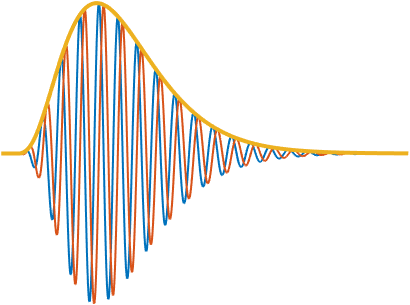
\includegraphics[height=2cm,width=3.5cm]{gammatone_Q8.png}}
 \put(2.5,0.0){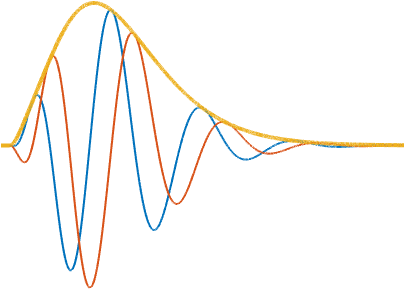
\includegraphics[height=2cm,width=3.5cm]{gammatone_Q1.png}}
\end{picture}
\caption{
\label{fig:gammatones}
Left: Gammatone wavelet $\boldsymbol{\psi_{\gamma_1}}(t)$ with a quality factor of $Q_1=8$.
Right: Gammatone wavelet $\boldsymbol{\psi_{\gamma_2}}(t)$ with a quality factor of $Q_2=1$.
\vl{we should discuss color schemes and axis labels}}
\end{center}
\end{figure}

Wavelets
$\boldsymbol{\psi_{\gamma_1}}(t)$ and $\boldsymbol{\psi_{\gamma_2}}(t)$ are designed as fourth-order Gammatone
wavelets with one vanishing moment \cite{Venkitaraman2014}, as shown in Figure \ref{fig:gammatones}.
In the context of auditory scene analysis, the asymmetric envelope of Gammatone wavelets is more biologically plausible than the symmetric, Gaussian-like envelope of the widespread Morlet wavelets.
Indeed, it allows to reproduce two important psychoacoustic effects in the mammalian cochlea: the asymmetry of temporal masking and the asymmetry of spectral masking \cite{Fastl2007}.
Moreover, it should be noted that Gammatone wavelets follow the typical amplitude profile of natural sounds, beginning with a relatively sharp attack and ending with a slower decay. \ml{tu peux citer le travail publié a Nature de lewicki, qui montrent que ces formes se retrouvent par ICA de sons naturels http://www.cs.cmu.edu/~learning/talks-2002/02-10-21.lewicki.pdf}


\section{Feature design}
Before supervised or unsupervised classification, it is beneficial to process scattering coefficients with feature transformations that improve invariance, normality, or generalization power. 
In this section, we review several ways of achieving these properties, namely binaural data augmentation, feature selection, logarithmic compression, standardization, and temporal integration.
The former has, to the best of our knowledge, not being considered for ASC and is specific to multichannel recordings, whereas the next ones would also apply to many other kinds of data.

\subsection{Feature selection by restricting the frequency range}
In a multivariate time series of descriptors $\mathbf{S}\boldsymbol{x}(t,\gamma)$, some coefficients $\gamma$ may consistently bear negligible information for the task of interest.
This fact may cause the classifier to overfit the training set, especially when the number of features is large and the number of training instances is small, as is the case here.
Selecting features appropriately before the training stage may circumvent this problem.
However, the parameters of the chosen feature selection algorithm are themselves prone to overfitting.
Instead, we adopt the more conservative approach of retaining all coefficients within a certain range of subband indices $\gamma_1$ and $\gamma_2$.
In comparison with adaptive algorithms, the subset of selected features $\gamma$ has a suboptimal statistical relevance, but it is easily interpretable in the realm of audio signal processing, as it is equivalent to a coarse band-pass filtering of $\boldsymbol{x}(t)$ and $\boldsymbol{x_1}(t,\gamma_1)$ over the time dimension $t$.

The conservation equations underlying the physics of sound production constrain the waveform $\boldsymbol{x}(t)$ to be regular in the time domain, that is, to have a polynomial decay in the Fourier domain.
This decay is only made sharper by the specific properties of acoustic environments, especially indoor.
Consequently, the amount of energy in the wavelet subband $\gamma_1$ is roughly inversely proportional to the center frequency $2^{-\gamma_1/Q_1}$.
In the topmost frequencies, this amount is so faint that the corresponding coefficients $\boldsymbol{x_1}(t,\gamma_1)$ and $\boldsymbol{x_2}(t,\gamma_1,\gamma_2)$ no longer bear discriminative information for the classification task at hand.

In the sequel, we evaluate the impact of discarding the scattering coefficients above a certain acoustic frequency $\xi_{1,\max}$, which corresponds to discarding subbands $\gamma_1$ below a certain scale
\begin{equation}
\gamma_{1,\min} =
\left\lfloor Q_1 \log_2 \frac{\xi_1}{\xi_{1,\max}} \right\rceil,
\end{equation}
where $\lfloor \cdot \rceil$ denotes a rounding to the nearest integer.

This strategy is already widespread in the literature.
For instance, we should note that \cite{roma2013}, who secured the first place in the 2013 edition of the DCASE challenge, rely on cepstral descriptors computed up to a cutoff frequency as small as $\xi_{1,\max}  = 900\,\mathrm{Hz}$ instead of the more conventional value of $16\,\mathrm{kHz}$.
\vl{Qu'en penses-tu ML ?}

\subsection{Logarithmic compression}
Many algorithms in pattern recognition, including nearest neighbor classifiers and support vector machines, tend to work best when all features follow a standard normal distribution across all training instances.
Yet, because of the complex modulus nonlinearity, scattering coefficients are nonnegative by design.
It appears empirically that their distribution is skewed towards the right, which means that the tail towards greater values is longer than the tail towards lower values.
However, skewness can be reduced by applying to all coefficients a pointwise concave transformation, \eg logarithmic.
Figure \ref{fig:histograms} shows the distribution of an arbitrarily chosen scattering coefficient over the DCASE 2013 dataset, before and after logarithmic compression.
\vl{Qu'en penses-tu ML ?}

\begin{figure}
\begin{center}
\setlength{\unitlength}{1cm}
\begin{picture}(5,2)
 \put(-1.5,0.0){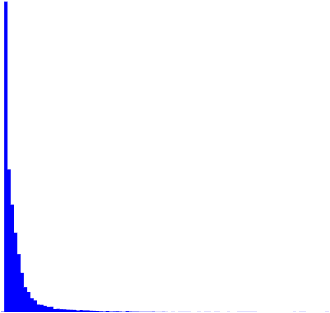
\includegraphics[height=2cm,width=3.5cm]{feature_histogram.png}}
 \put(2.5,0.0){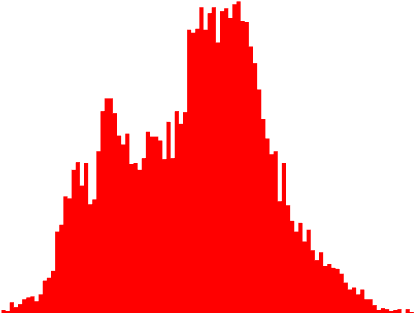
\includegraphics[height=2cm,width=3.5cm]{feature_histogram_logcompressed.png}}
\end{picture}
\caption{
\label{fig:histograms}
\vl{we should discuss color schemes and axis labels}}
\end{center}
\end{figure}

The application of the pointwise logarithm to magnitude spectra is ubiquitous in audio signal processing.
Indeed, it is corroborated by the Weber-Fechner law in psychoacoustics, which states that the sensation of loudness is roughly proportional to the logarithm of the acoustic pressure.
We must also recall that the measured amplitude of sound sources often decays polynomially with the distance to the binaural microphone, which is a spurious factor of variability to the task of auditory scene classification.
Logarithmic compression can linearize this dependency, which arguably facilitates the construction of a powerful invariant at the classifier stage.

Given a task of musical genre recognition, \cite{Anden2014} has advocated for the renormalization of second-order scattering coefficients $\mathbf{S_2}\boldsymbol{x}(t,\gamma_1,\gamma_2)$ by the corresponding first-order scattering coefficients $\mathbf{S_1}\boldsymbol{x}(t,\gamma_1)$, as it provably decorrelates the amplitudes of their activations.
Interestingly, taking the logarithm of renormalized coefficients would yield
\begin{equation}
\log \dfrac{\mathbf{S_2}\boldsymbol{x}(t,\gamma_1,\gamma_2)}{\mathbf{S_1}\boldsymbol{x}(t,\gamma_1)} =
\log \mathbf{S_2}\boldsymbol{x}(t, \gamma_1, \gamma_2) -
\log \mathbf{S_1}\boldsymbol{x}(t, \gamma_1),
\end{equation}
\ie a linear combination of the logarithms of first- and second-order coefficients.
Therefore, the theoretical insight brought by \cite{Anden2014} in favor of renormalized scattering also applies to log-scattering up to a linear transformation in feature space, to which affine classifiers are not sensitive.

\subsection{Early \vs late temporal integration}
Owing to the scarcity of salient events in many natural scenes,
fine-grained classification is only made
possible by integrating signal information over a long temporal context.
Indeed, whereas a few seconds are often sufficient to recognize a speaker,
a musical instrument, or a genre, it may require up to 30 seconds
to disambiguate two classes auditory scenes which share part of their semantic content, \eg a train from a subway station or a quiet street from a park.
Depending on whether aggregation is performed in feature space or in decision space, the corresponding method is referred to as early or late integration.

A straightforward application of early integration consists in summarizing the multivariate time series of scattering coefficients over the full duration of the auditory scene, by retaining their average values only.
Going back to the definition of the scattering transform given in section \ref{sec:scattering}, this is equivalent to increasing the support $T$ of the low-pass filter $\boldsymbol{\phi}(t)$ up to infinity. With a slight abuse of notation, we denote by
\begin{equation}
\mathbf{S}\boldsymbol{x}(\gamma) =
\int_{-\infty}^{+\infty} \mathbf{S}\boldsymbol{x}(t,\gamma)\;\mathrm{d}t
\end{equation}
the summarized features.

Conversely, a late integration scheme relies on probabilistic estimates over short-term windows of length $T$, which are subsequently aggregated to produce a final decision
\begin{equation}
\hat{y} = \arg \max_{y} \rho\Big(\big\{ \mathbb{P}\left[y \,\vert\, \mathbf{S}\boldsymbol{x}(t,\gamma) \right] \big\}_{t} \Big),
\end{equation}
where $\hat{y}$ is the estimated class label and $\rho$ is a reduction function, such as sum, product, or majority vote \cite{Kittler1998}.

The principal drawback of early integration is that it drastically reduces the number of training instances at the classifier stage, down to one per auditory scene -- if data augmentation is not considered.
In the context of the DCASE 2013 dataset, this corresponds to merely $8$ training instances per class, and $80$ instances overall, hence an increase in variance in statistical estimation and a risk of overfitting.
On the contrary, a late integration scheme for $T=188\textrm{ ms}$ would yield $128$ instances per auditory scene, resulting in $10240$ instances overall.
However, many of these instances may be silent or lack any salient properties of the class they are assigned to, hence an increase in bias and a risk of underfitting.
In short, early and late integration methods lie at opposite ends of the bias-versus-variance statistical tradeoff. We refer to \cite{Joder2009} for a comprehensive review of this problematic in the context of musical instrument recognition.

\subsection{Standardization}
Let $\mathbf{S}\boldsymbol{X}(\gamma,n)$ be a dataset, where the indices $\gamma$ and $n$ respectively denotes features and examples.
It is commonly acknowledged that support vector machines should be trained on scaled features with null mean and unit variance, so as to avoid mismatch in numeric ranges.
This operation may also help making the dataset linearly separable in feature space.
\vl{Check this claim in DCASE 2013 time scattering features.}
To standardize $\mathbf{S}\boldsymbol{X}(\gamma,n)$, we apply the affine transformation
\begin{equation}
\widetilde{\mathbf{S}}\boldsymbol{X}(\gamma, n) =
\dfrac{ \mathbf{S}\boldsymbol{X}(\gamma, n) -
\mathbb{E}[ \mathbf{S}\boldsymbol{X}](\gamma)}{\sigma[ \mathbf{S}\boldsymbol{X}](\gamma)}
\end{equation}
where $\mathbb{E}[ \mathbf{S}\boldsymbol{X}](\gamma) = \frac{1}{N} \sum_{n=1}^{N} \mathbf{S}\boldsymbol{X}(\gamma,n)$ is the expected value of $\mathbf{S}\boldsymbol{X}(\gamma,n)$ and
\begin{equation}
\sigma[\mathbf{S}\boldsymbol{X}] (\gamma) =
\sqrt{\frac{1}{N-1} \sum_{n=1}^{N}
\left( \mathbf{S}\boldsymbol{X}(\gamma,n) - \mathbb{E}[\mathbf{S}\boldsymbol{X}] \right)^2}
\end{equation}
 is the sample standard deviation.
 
 The vectors $\mathbb{E}[\mathbf{S}\boldsymbol{X}(\gamma)]$ and $\sigma[\mathbf{S}\boldsymbol{X}](\gamma)$ are estimated from the training set only, and the same affine transformation is subsequently applied to all samples in the training set and the test set.
 
The next section discusses adaptive methods for the temporal integration of scattering coefficients in an unsupervised setting.

\section{Object-based modeling of the scene}

It has been shown the perception of complex acoustic scene rely on the identification of putative sound sources.
\ml{GL 2 colonnes}

describe in terms of high level attributes

be they cognitive ones such as pleasantness, or descriptive ones such as the type of environment where the 


%As part of the aforementioned research areas and applications, the emerging field of \emph{Acoustic Scene Analysis} (also called \emph{Sound Scene Analysis}) \cite{Stowell15} aims to develop approaches and systems for the automatic analysis of environmental sounds and soundscapes (originating both from urban or nature environments). While research methodologies in related fields such as Automatic Speech Recognition (ASR) \cite{Rabiner93} and Music Information Retrieval (MIR) \cite{Muller07} are now well established, research addressing Acoustic Scene Analysis remains relatively young. 

Whilst the range of applications are very large, so is the need

holistic / event based

skeleton of events on a bed of texture.

debate about the kind of process underlying perception

strong indication that the detection of specific events, named markers suffice to trigger class prediction

From a numerical data processing overview, the holistic scheme as a simplicity, but clearly face poor performance on realistic conditions \cite{lagrange:hal-01082501}.

If available, the complete description of the scene in terms of event occurrences is powerful enough to reliably predict high level cognitive classes, \textit{i.e.} the presence of birds are strong pleasantness indicators and very likely to be heard in parks in urban areas.

To take into account this object-based representation, we propose the following 3-steps algorithm:

\begin{itemize}
\item step 1: features extraction.
\item step 2: scene-wise clustering step. A clustering is performed on each scene using an enhanced version of the popular K-means algorithm known as K-means$++$ \cite{arthur2007k}, which differs from k-means method in terms of selection of starting points. Each scene is then describe with a set of centroids.
\item step 3: Centroids similarity. The similarity between the centroids is computed using a radial basis function kernel $K^c$ as well as the local scaling method proposed in \cite{selfTuneManor2004}: \\
\begin{equation}
\begin{split}
K^c_{ij} & =exp\left( - \dfrac{\parallel x_i - x_j \parallel^2}{\sigma_{i}\sigma_{j}} \right) \\
\sigma_{i} & =\parallel x_i - x_N \parallel
\end{split}
\end{equation}

with $x_N$ the $N$'th nearest neihgbor of the centroid $x_i$. \\

\item step 4: scene similarity \\
\end{itemize}

To compute the scene similarity based on the extracted centroids, we propose the three following strategies:

\begin{itemize}
\item \emph{closest}: the similarity between two scenes is equal to the largest similarity between their centroids.
\item \emph{averaged}: the similarity between two scenes is equal to the average of their centroids similarities.
\item \emph{weighted}: for each scene, each centroid is weighted according to the number of frames belonging to its cluster. 
\end{itemize}

To compute the  weighted similarity between two scenes by taking into account both theirs clusters weights and theirs centroids similarities, we use a variant of the Earth Moving Distance ($EMD$) adapted for non-normalized histograms known as $\widehat{EMD}$ \cite{pele2008linear} with the implementation proposed in  \cite{pele2009fast}. Considering two histograms $h_i$ and $h_j$, represented the centroids weights of each scene, the $\widehat{EMD}$ is computed as follow:

\begin{equation}
\begin{split}
\widehat{EMD}(h_i,h_j) &=( \min\limits_{f_{ij}} \sum\limits_{i,j} f_{ij}D_{ij} )  \\ 
&+ \mid \sum\limits_{i} h_i - \sum\limits_{j} h_j  \mid \alpha \max\limits_{i,j} D_{ij}
\end{split}
\end{equation}

\begin{equation*}
s.t. \quad f_{ij}\geq0\quad \sum\limits_{j} f_{ij} \leq h_{i}\quad \sum\limits_{i} f_{ij} \leq h_{j} 
\end{equation*}
\begin{equation*}
\sum\limits_{i,j}f_{ij} = \min( \sum\limits_{i} h_{i} ,\sum\limits_{j} h_{j} )
\end{equation*}

where $f_{ij}$ is the flow, and $D_{ij}$ is the ground distance. In our case the ground distance is $1-K^c_{ij}$ 

To get the final similarity measure between two scenes $s_i$ and $s_j$, we use an extended Gaussian kernels $K^s$ (Chapelle et al., 1999; Jing et al., 2003).

\begin{equation*}
K^s(s_i,s_j) = exp\left( - \dfrac{\widehat{EMD}(h_i,h_j)}{A} \right) \\
\end{equation*}

with $A$ a scaling parameter, set to the mean value of the $\widehat{EMD}$. \\

The resulting kernel is an EMD kernel. It has to be noted that there is no proof that such kernel is positive definite.

\section{Experimental Evaluation}

\subsection{Acoustic Scene Similarity and Classification}

The object-based approach is assessed considering both an ASS and an ASC scenario:

\begin{itemize}
\item \emph{ASS}: It is an unsupervised scenario. Evaluation is performed on the private dataset of the DCASE 2013 challenge, using the precision at rank $k$ ($k=[3,\ldots,9]$) metrics. Similarity between scenes features is then computed using a Gaussian kernel with local scaling. 

\item \emph{ASC}: It is a supervised scenario. The systems are evaluated  with five-fold  stratified cross validation on the  private dataset of the DCASE 2013 challenge. The folds are identical to those used in the original challenge. A linear Support Vector Machine (SVM) is used as classifier. For object-based approach, we only consider the step 2. Consequently, each scene is represented by a set of centroids and each centroid is classified separately. The final scene classification is based on a majority vote. In this case, the object-based approach may be seen as a mid integration strategy.
\end{itemize}

The object-based approach is compared to standard approaches using early integration strategy for the ASS scenario, and both early and late integration strategies for the ASC scenario (see Section \ref{XX}). 

\subsection{Features}

Two features are used to describe the scenes: temporal-scattering and Mel Frequency Cesptral Coefficients (MFCCs). For the temporal-scattering, each scene is described by 128 vectors of scattering coefficients. A logarithm compression (see Section\ref{XX}) is applied to the temporal-scattering coefficient. Different set of parameters were tested to compute the MFFCs, we here present only the results for the best setting, that is, 40 MFCCs (including the 0 energy coefficient) computed for windows of 50ms and hops of 25ms, with a limited frequency range of $27.5-1000$Hz. This setting gives us 600 feature vectors per scenes. To reduce the data dimensionality, a pooling step is performed on the MFCCs vectors: each set of MFCCs vectors is dividing into $n$ non-overlapping $t$-seconds long slices. Each $n$ MFCC slices is then averaged over time. To ensure that each scene is described by circa the same number of vectors for both the temporal-scattering and the MFCCs, we set $t$ to 250ms, giving us 120 MFCCs vectors per scenes. 

\section{Acoustic Scene Similarity}

\subsection{Role of logarithmic compression}

\subsection{MFCC \vs Time scattering}

\subsection{Object-based \vs early integration}

\section{Acoustic Scene Classification}
Support vector machines are large-margin binary discriminators with tunable regularization of misclassified examples.

\subsection{Role of logarithmic compression}

\subsection{MFCC \vs Time scattering}

\subsection{Object-based \vs early/late integration}

\section{Conclusion}

In this paper, the benefit of considering 1) the scattering transform for building discriminant features and 2) unsupervised clustering for the modeling of large time span environmental acoustic scenes. Experiments shows that the time/frequency scattering achieves better discriminability than the time scattering one or MFCCs as they probably better isolate elements of interest in different information channels, thus allowing an efficient and scalable early integration process. This leads to improvement both for the ASSR and ASC tasks.

Abstracting the scene as a reduced set of exemplars with adapted similarity strategies allows us to improve ASSR performance when the BOF approaches based on GMMs fails with reference to an early integration scheme. Those results advocate for a hierarchical model of the scene, where small time scale structure  (below a second) shall be decorelated using convolutional network such as the ones of the scattering transforms and larger time scale (over a second) structure shall be modeled as adaptive aggregates that can be identified in the time domain in an unsupervised setting and in the features domain in the supervised case (provided that the dimensionality is sufficiently high). 

This assertion shall be challenged in future work by considering larger databases and more diverse application scenarios, such as pleasantness prediction \cite{acta} or ecoacoustics tasks.

\bibliographystyle{unsrt}
\bibliography{biblio}

% biography section
% 
% If you have an EPS/PDF photo (graphicx package needed) extra braces are
% needed around the contents of the optional argument to biography to prevent
% the LaTeX parser from getting confused when it sees the complicated
% \includegraphics command within an optional argument. (You could create
% your own custom macro containing the \includegraphics command to make things
% simpler here.)
%\begin{IEEEbiography}[{\includegraphics[width=1in,height=1.25in,clip,keepaspectratio]{mshell}}]{Michael Shell}
% or if you just want to reserve a space for a photo:

%\begin{IEEEbiography}{Mathieu Lagrange}
%Biography text here.
%\end{IEEEbiography}

% if you will not have a photo at all:
%\begin{IEEEbiographynophoto}{John Doe}
%Biography text here.
%\end{IEEEbiographynophoto}

% insert where needed to balance the two columns on the last page with
% biographies
%\newpage

%\begin{IEEEbiographynophoto}{Jane Doe}
%Biography text here.
%\end{IEEEbiographynophoto}

% You can push biographies down or up by placing
% a \vfill before or after them. The appropriate
% use of \vfill depends on what kind of text is
% on the last page and whether or not the columns
% are being equalized.

%\vfill

% Can be used to pull up biographies so that the bottom of the last one
% is flush with the other column.
%\enlargethispage{-5in}



% that's all folks
\end{document}


